\section{Systemarkitektur}
\begin{figure}
\label{fig:sysArk}
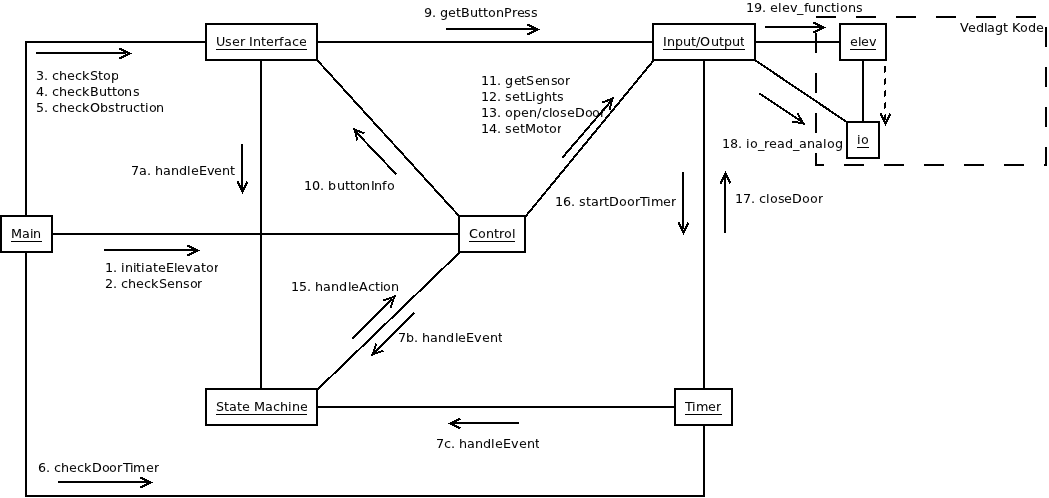
\includegraphics[width=\textwidth]{systemarkitektur.png}
\caption{Overordnet systemarkitektur}
\end{figure}
\begin{enumerate}
\item initiateElevator kalles hver gang programvaren starter opp, for å definere heisen.
\item checkSensor sjekker sensoren.
\item checkStop sjekker stoppknappen.
\item checkButtons sjekker for bestillinger.
\item checkObstruction sjekker for obstruksjon.
\item checkDoorTimer sjekker dørtimeren.
\item handleEvent kalles i tre klasser, når forskjellige hendelser oppstår.
	\begin{enumerate}
	\item den kalles i ui-klassen når en knapp blir trykket inn, slik at bestillingen blir registrert i ordrelisten, eventuelt håndterer en nødstopp. Den sjekker også om en obstruksjon blir fjernet, slik at heisen eventuelt kan begynne å kjøre.
	\item i control-klassen genereres det en hendelse når  heisen ankommer en etasje, slik at heisen kan avgjøre om den skal stoppe eller ikke. Den kalles også når en ny ordre kommer inn.
	\item Den siste klassen som kaller handleEvent-funksjonen er timer-klassen. Den genererer en hendelse når døren lukkes. 
	\end{enumerate}
\item handleAction kalles hver gang tilstandsmaskinen får et kall på handleEvent, og det er spesifisert en handling for denne nåtilstanden og hendelsen.
	\begin{enumerate}
	\item handleEmergencyStop kalles når heisen enten får stoppsignal gjennom stoppknappen, eller at den får inn obstruksjon mellom etasjene.
	\item \label{handleDestination} handleDestination setter en ny retning for heisen, og starter motoren
	\item \label{handleDestinationFromIdle} handleDestinationFromIdle gjør det samme som \ref{handleDestination}, men denne sjekker først om bestillingen kommer fra nåværende etasje. Dette er nødvendig siden heisen står med dørene lukket, og må følgelig åpne de dersom den har en ordre i nåværende etasje, før den kjører videre.
	\item handleDestinationFromEM starter motoren fra nødstopptilstanden. Denne vil, i tillegg til det samme som \ref{handleDestinationFromIdle}, også slukke stopplyset.
	\item handleStop sørger for at heisen stoppper og åpner døra når den har en ordre i en etasje. Den fjerner også de aktuelle ordrene i etasjen.
	\item handleNewOrder sørger for å legge inn alle bestillinger som gjøres, og setter respektive lys.
	\end{enumerate}
\item getButtonPress sjekker IO-klassen, og henter informasjon om hvilken knapp som ble trykket inn sist.
\item buttonInfo henter informasjon om hvilken bestillingsknapp som ble trykket inn sist, for å legge inn rett ordre.
\item getSensor henter informasjon om hvilken etasje heisen er i.
\item setLights er et samlebegrep for alle funksjoner som setter lys
\item openDoor og closeDoor håndterer døra.
\item setMotor håndterer motoren.
\item startDoorTimer kalles når døra åpnes for å telle ned tre sekunder.
\item closeDoor kalles fra timer-klassen når timeren har telt ned.
\end{enumerate}
